
\begin{decision}
一般情况下,答辩委员会决议的内容不宜过少,亦不宜超过一页。不同学院对此页的要求(是否需要包含此页在最终存档模板内,是否需要单独提交,包含在模板内的改页是否需要答辩主席签字等)可能有所不同,具体内容请参照学院的相关规定。 

若不需要此页,请将其从模板中删除。删除方式为注释或去掉本环境。
\end{decision}



\begin{publications}
    已发表论文:
    \renewcommand{\labelenumi}{[\arabic{enumi}]}
    \begin{enumerate}
        \item {
            \textbf{Xinze Zhang}, Kun He, and Yukun Bao. Error-feedback Stochastic Modeling Strategy for Time Series Forecasting with Convolutional Neural Networks. Neurocomputing, 2021, 459:234-248.(SCI 源刊,IF 5.719,署名单位:华中科技大学)
              }
        \item {Jianhua Yang, \textbf{Xinze Zhang}, and Yukun Bao. Short-term Load Forecasting of Central China based on DPSO-LSTM. In Proceedings of IEEE 4th International Electrical and Energy Conference, IEEC 2021. (EI 会议,署名单位:华中科技大学)
              }
        \item {\textbf{Xinze Zhang}, Junzhe Zhang, Zhenhua Chen, and Kun He. Crafting Adversarial Examples for Neural Machine Translation. In Proceedings of the 59th Annual Meeting of the Association for Computational Linguistics, ACL 2021. (CCF A类国际会议,署名单位:华中科技大学)}
    \end{enumerate}

    \vspace{1em}
    工作论文:
    \begin{enumerate}
        \item {
            \textbf{Xinze Zhang}, Kun He, Yukun Bao, and Qi Sima. Error-feedback Triple-phase Optimization to Configurable Convolutional Echo State Network for Time Series Forecasting.
              }
        \item {
            \textbf{Xinze Zhang}, Qi Sima, Kun He, Yukun Bao, and Shuhan Chen. Enhancing Echo State Network with Particle Swarm Bayesian Optimization Enabled Echo State Selection for Time Series Forecasting.
              }
        \item {
             Qi Sima, \textbf{Xinze Zhang}, and Yukun Bao. Reinforced Decoder: Towards Training Sequence-to-Sequence Model for Time Series Forecasting.
              }
    \end{enumerate}

\end{publications}

\begin{paperRelation}
    \renewcommand\tabularxcolumn[1]{m{#1}}
    % 已发表论文与博士学位论文的关系:
    \begin{table}[!htbp]
        \centering
        \renewcommand\arraystretch{2}
        \begin{tabularx}{\textwidth}{|c|Y|Y|Y|Y|}
            \hline
            \makecell*[c]{序号} & \makecell*[c]{成果名称}                                                                                      & \makecell*[c]{成果形式} & \makecell*[c]{成果主要内容} & \makecell[c]{与学位论文 \\对应关系} \\ \hline
            1                   & {Error-feedback Stochastic Modeling Strategy for Time Series Forecasting with Convolutional Neural Networks} & \makecell[c]{SCI 期刊                                                           \\(已发表)}    &  \multicolumn{1}{X|}{提出了误差反馈随机建模的迭代构造策略,结合贪心搜索自适应确定卷积结构,构造出一种新颖、高效且准确的随机卷积神经网络预测模型}     &   \multicolumn{1}{X|}{该成果为论文第3章主要内容}         \\ \hline
            2                   & {Short-term Load Forecasting of Central China based on DPSO-LSTM}                                            & \makecell[c]{EI会议                                                             \\(已发表) }    &  \multicolumn{1}{X|}{提出了时步多维度的时序输入特征二维结构,结合粒子群优化算法选择时步维度与模型参数,提升了LSTM模型的短期电力负荷预测效果}        & \multicolumn{1}{X|}{基于对该成果的改进,构成论文第5章主要内容}         \\ \hline
        \end{tabularx}
    \end{table}
\end{paperRelation}

\begin{project}
    \renewcommand{\labelenumi}{\arabic{enumi}.}
    \begin{enumerate}
        \item {国家自然科学基金面上项目:大数据环境下基于计算智能的预测建模技术及其在电力负荷预测中的应用,批准年限:{2019/01 - 2022/12}。}
        \item {国家自然科学基金面上项目:{自然语言处理深度模型的对抗攻防关键算法研究,批准年限:{2021/01 - 2024/12}}。}
        \item {湖北省国际科技合作项目:{深度学习模型对抗攻防基础理论与算法研究,批准年限:{2021/09 - 2023/09}}}。
        \item {国家电网公司科技项目:{华中区域共享型电力交易与服务平台关键技术研究,批准年限:2020/06 - 2021/11}}。
        \item {国家电网公司科技项目:{渝鄂直流运行条件下华中消纳西南水电交易电量库模型建立与效益分析,批准年限:2019/05 - 2020/11}}。
    \end{enumerate}

\end{project}

\begin{denotation}
\item[CNN] Convolutional Neural Network(卷积神经网络)
\end{denotation}


\begin{otherDatas}
    % 其他数据图表或程序
    本处放置其他数据图表或程序的相关内容。当仅包含某一类别时,建议将本节名进行修改。例如,本节将仅包含本论文中所使用的数据集图示,因此在本人所提交的学位论文中,基于答辩委员会的意见,本节名称被修改为“本文数据集展示”。 若无其他数据图表或程序,建议将本节删除。删除方式为注释或去掉本环境。
    
    以下是本节内容节选:

    \cref{fig:app.ar1}展示了本文中的经典人工合成时间序列数据,包括一阶自回归(AR1)合成数据.....各数据集的简要说明如下:

    \autoref{fig:app.ar1}展示了AR1合成数据,该数据参考相关研究\cite{qi2008trend,crone2016feature}的参数设定,通过\autoref{sec:esm.exp}中的\autoref{eq:ar}予以合成。

    \begin{figure}[h]
        \centering
        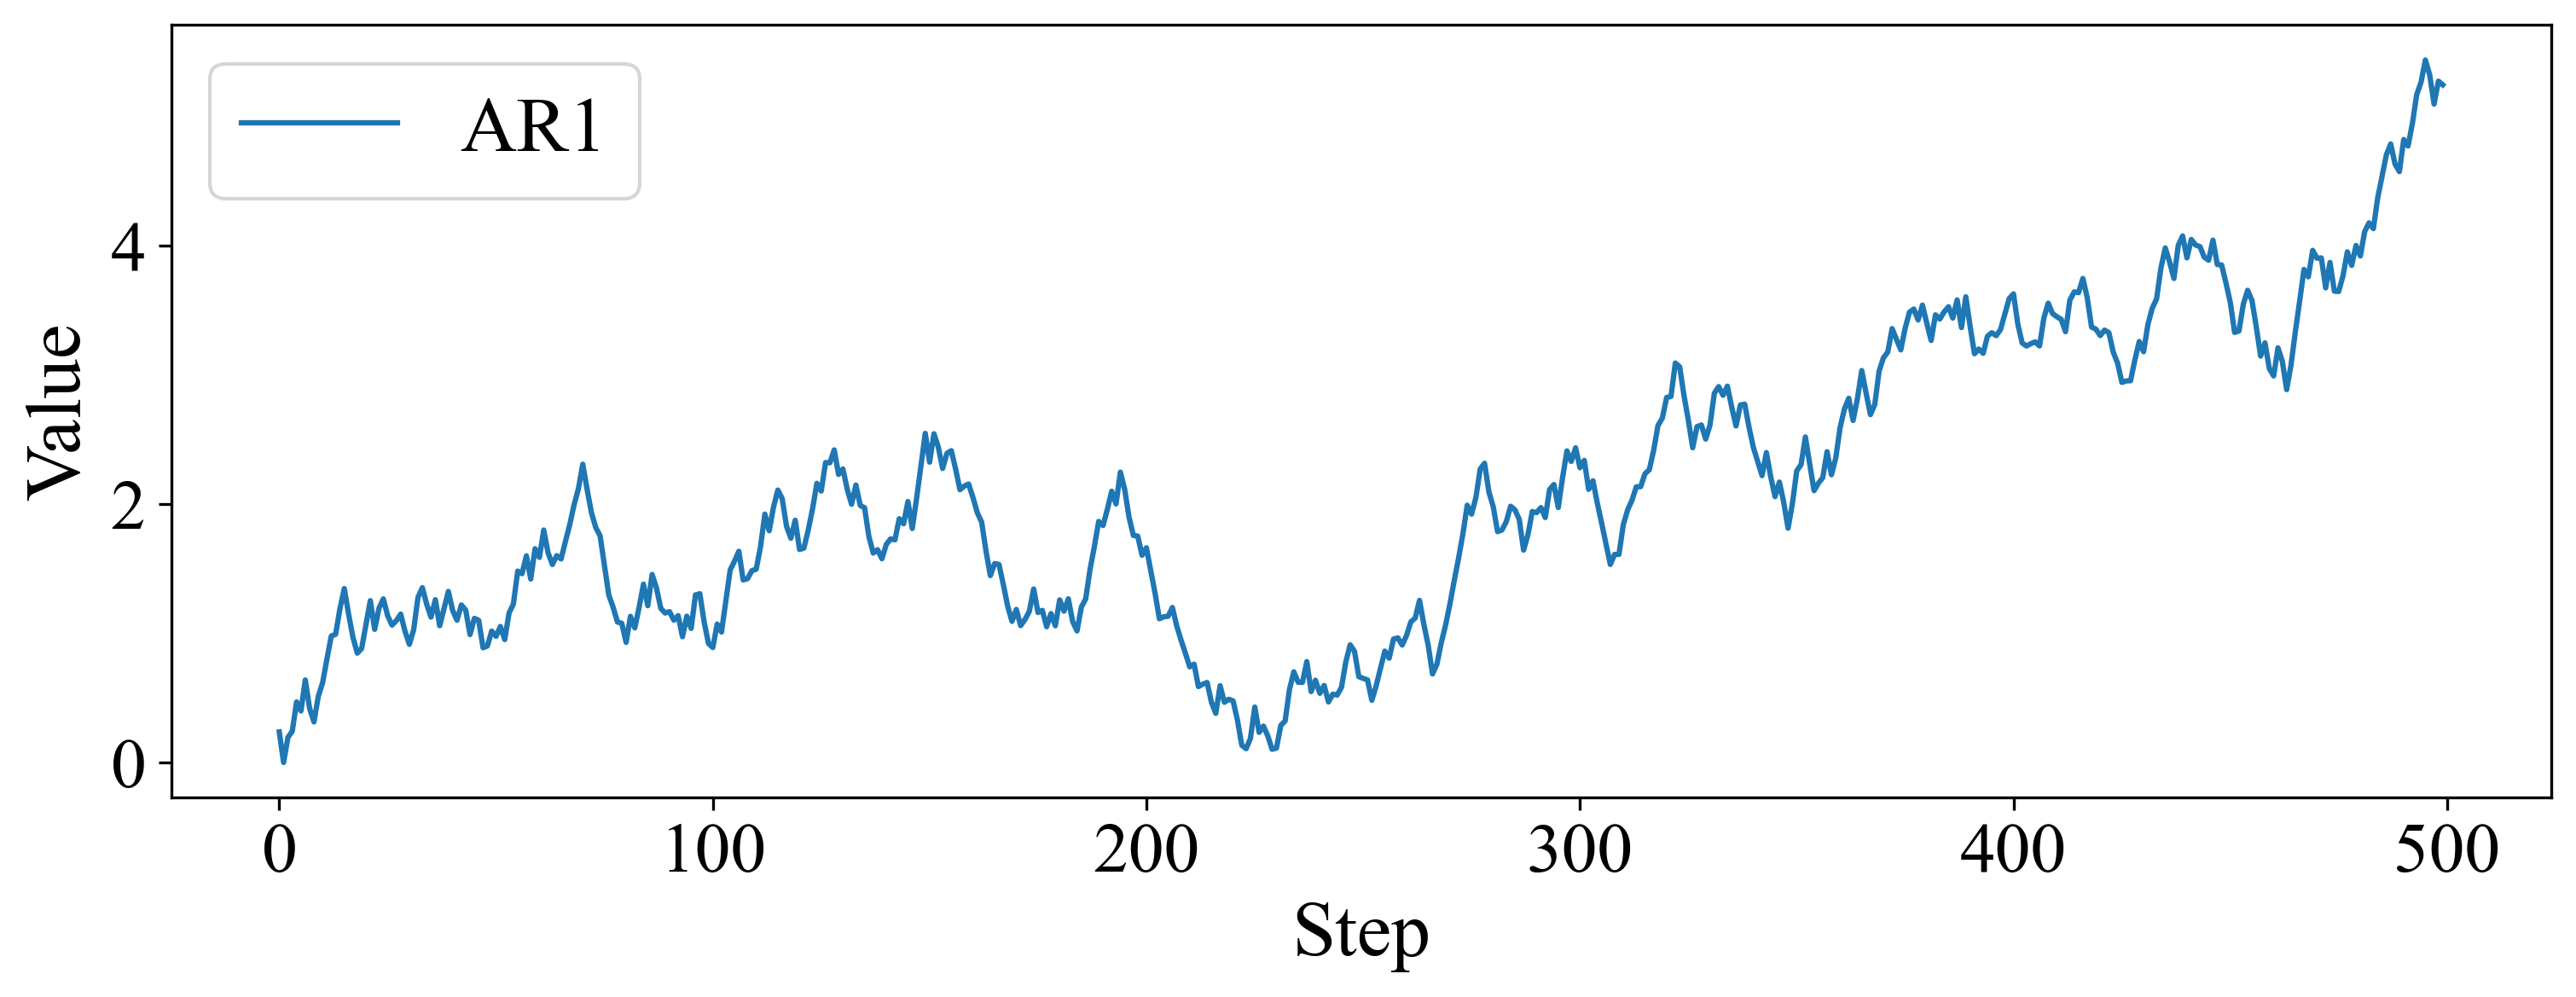
\includegraphics[width = 0.9\textwidth]{float/ch.app/ar1.png}
        \captionsetup{skip=2pt}
        \setlength{\belowcaptionskip}{-8pt}
        \caption{AR1合成数据\label{fig:app.ar1}}
    \end{figure}
    
\end{otherDatas}
% \phantomsection
% \input{body/chapter/univ.tex}